%% mainpart.tex
%%

%------------------------------------------------------------------------------------------------
\section{Analyse der Datenschutz-Konformität}
\label{sec:Analyse der Datenschutz-Konformität}
%------------------------------------------------------------------------------------------------

Basierend auf den eingeführten Grundlagen aus \fullref{sec:Grundlagen} wird nachfolgend das Erheben der Daten im Rahmen der smarten Umgebungen \textbf{Smart Home} und \textbf{Smart City} betrachtet. Darauf aufbauend erfolgt eine kritische Auseinandersetzung hinsichtlich ihrer Konformität im Rahmen der \ac{dsgvo}, die in eine Vorstellung möglicher Handlungsempfehlungen und Optionen übergeht, die es den Nutzern ermöglichen soll, nach eigenem Ermessen die Erhebung der von ihren Geräten gesammelten Daten zu regulieren oder dementsprechende Vorkehrungen zu treffen, die über sie gesammelten Daten zu minimieren. Abschließend erfolgt eine Bewertung der gesammelten Ergebnisse mit einhergehender Beantwortung der aufgestellten \acl{rq}.

%%------------------------------------------------------------------------------------------------
%\subsection{Datenerhebung}
%\label{sec:Hauptteil:ssec:Datenerhebung}
%%------------------------------------------------------------------------------------------------
%
%Beginnend mit der Analyse der Datenerhebung anhand der einzelnen Geräte in den vorliegenden Kontexten. Die Wahl von \textbf{Smart City} und \textbf{Smart Home} als Gegenstand der Analyse wurde aufgrund der hohen Interaktionsrate zwischen den einzelnen Geräten und den \textbf{ds} gewählt. Neben Smart TVs, Smart Watches und Sensoren interagieren die Nutzer fast minütlich mit den entsprechenden Geräten.
%
%%------------------------------------------------------------------------------------------------
%\subsubsection{Smart Home}
%\label{sec:Hauptteil:ssec:Datenerhebung:sssec:Smart Home}
%%------------------------------------------------------------------------------------------------

\noindent \textbf{Smart Home.}
Die Analyse der erhobenen Daten aus dem Bereich des Smart Home wird anhand der Veröffentlichungen \cite{Mandalari2021,Ren2019} durchgeführt. Fokus der beiden wissenschaftlichen Arbeiten war die Analyse der Dienstbereitstellung und der damit verbundenen Daten, die ausgehend von den \textbf{Smart Devices}, über das Netzwerk gesendet werden. Mittels dieser zugrundeliegenden Informationen konnte eine Betrachtung hinsichtlich der Einhaltung derzeit geltender Datenschutzrichtlinien durchgeführt werden.
Da es sich bei den beiden angesprochenen Arbeiten um zwei voneinander unabhängige Experimente handelt, werden die Vorgehensweisen und die jeweiligen Resultate zur besseren Verständlichkeit separiert in...
\begin{itemize}
	\item \textbf{Projekt 1}: Analyse des Datenverkehrs für die Bereitstellung der Dienste
	\item \textbf{Projekt 2}: Analyse der Daten und deren geolokalen Ziele
\end{itemize}
\noindent ... dargestellt.

\noindent Beginnend mit der Zielsetzung von \textbf{Projekt 1}, das Identifikation von essenziellem Datenverkehr zur Bereitstellung der jeweiligen Dienste des \ac{iot}-Gerätes als Forschungsthema definiert. Die hierbei analysierten Geräte und Anwendungen können im Kontext von Smart Home den Typen \textbf{Kamera}, \textbf{Heimautomatisierung}, \textbf{Smart-Hubs}, die mehrere Geräte innerhalb eines smarten Netzwerkes miteinander verbinden können, \textbf{Smart Speaker} und \textbf{Video} zugeordnet werden. Die hiermit aggregierte Grundgesamtheit von 31 Geräten wurde anschließend innerhalb einer Testumgebung mit isoliertem Netzwerk installiert und über automatisierte Trigger-Funktionen getestet. Neben maschinellen Eingaben über die zur Verfügung gestellten Schnittstellen (Smartphone-Applikationen und Webseiten) sind aufgenommene Sprachbefehle für das Testen der Sprachassistenten verwendet worden. Hiermit wurden basierend auf mehreren Durchläufen die einzelnen Funktionen der Geräte isoliert ausgelöst und über Packet Dumps an den vorgeschalteten Routern mitgeschnitten.
Der exemplarische Aufbau der Testumgebung und der Durchführung der einzelnen Messungen kann anhand nachfolgender Abbilding \ref{fig:test-setup-proj1} beschrieben werden.
\begin{figure}
    \centering
    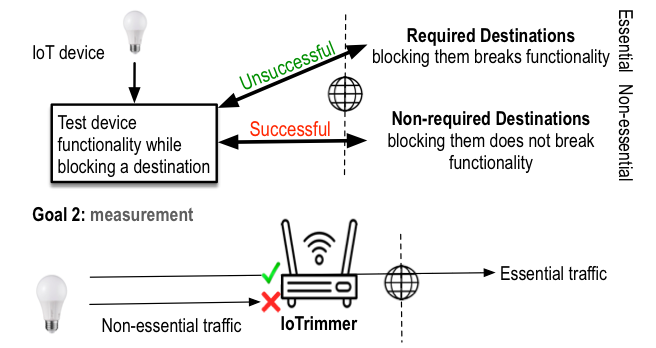
\includegraphics[scale=0.4]{main/pictures/countermeasures/IoTrimmer_IoTrigger}
    \caption{High-Level Architektur der Testumgebung für die Analyse des Netzwerkverkehrs der \ac{iot}-Geräte auf Basis von \textbf{Projekt 1} \cite{Mandalari2021}}
    \label{fig:test-setup-proj1}
\end{figure}

\noindent Die Identifikation der nicht essenziellen Endpunkte, die weder für die Bereitstellung der Service-Funktionalität des Gerätes verwendet werden noch für den Verwender von Nutzen sind, wurde auf Basis selbstentwickelter Werkzeuge in Form von Skripten, die auf den Routern der Testumgebung platziert wurden, durchgeführt. Eine genauere Betrachtung und Erläuterung der Funktionsweise dieser Werkzeuge folgt im späteren Verlauf dieser Ausarbeitung als Bestandteil der Sektion \fullref{sec:Hauptteil:ssec:Regulationsmöglichkeiten} im Rahmen der Auswertung von Präventionsmöglichkeiten von nicht datenschutzkonformen Aktivitäten der Geräte im Smart Home.
Mittels dieses Experimentes konnte basierend auf den Funktionen der 31 getesteten Geräte eine Teilmenge von 16 Geräte identifiziert werden, die Daten an mindestens eine nicht benötigte Adresse zur Dienstbereitstellung senden. Die maximale Anzahl an blockbaren nicht benötigten Endpunkten lag im Kontext der ersten Untersuchung der Geräte bei elf Endpunkten. Diese Ergebnisse werden als Teil der nachfolgenden Grafik \ref{fig:result-non-req-dest} nochmals in Form eines Balken-Diagramms separiert der einzelnen Geräte-Typen dargestellt.
\begin{figure}
    \centering
    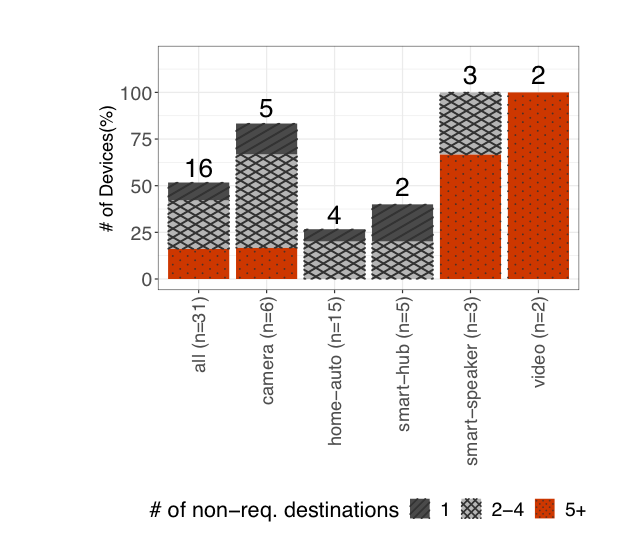
\includegraphics[scale=0.3]{main/pictures/projekt_one/Non_Required_Traffic}
    \caption{Ergebnisse der Analyse und Kategorisierung des Netzwerkverkehrs in essenziellen und nicht essenziellen Datenverkeht von \textbf{Projekt 1} auf Basis von \cite{Mandalari2021}}
    \label{fig:result-non-req-dest}
\end{figure}

\noindent Nach der Kategorisierung des gesammelten Netzwerkverkehrs wurde dieser anschließend nochmals in Kategorien bezüglich seiner finalen Ziele unterteilt. Die Unterscheidung wurde auf Basis von \textbf{First-Party}, \textbf{Support-Party} und \textbf{Third-Party} in Verbindung mit den aufgelösten Hostnamen vorgenommen, die nachfolgend nochmals genauer definiert werden.
\begin{itemize}
	\item \textbf{First-Party} sind Service-Endpunkte, die von den Geräteherstellern selbst bereitgestellt werden
	\item \textbf{Support-Party} beschreiben Endpunkte, die Support-Dienstleistungen für die einzelnen Geräte zur Verfügung stellen. Hierunter fallen beispielsweise Überwachung des Gerätestatus, Identifikation von Fehlfunktionen oder die Bereitstellung von Rechenkapazität für die Anwendungen.
	\item \textbf{Third-Party} Endpunkte sind wiederum Werbe- oder Marketing-Unternehmen, die die gesendeten Daten für marktanalytische Zwecke nutzen.
\end{itemize}

\noindent Resultierend aus dieser feingranulareren Unterteilung des Netzwerkverkehrs in die drei beschriebenen Kategorien, konnte die Erkenntnis gewonnen werden, dass beispielsweise der Datenverkehr an Endpunkte aus dem Bereich \textbf{Third-Party} nie für die Bereitstellung der Standardfunktionen eines \ac{iot}-Gerätes verwendet wird. Dieses Ergebnis wird nachfolgend nochmals in Form eines Balkendiagramms \ref{fig:result-non-req-dest-per-party} dargestellt, dass die Anzahl an Endpunkten gegen die fünf analysierten Geräte-Kategorien beschreibt. Hierbei kann in notwendige (rechts) und nicht notwendige Endpunkte (links) unterschieden werden. 
\begin{figure}
    \centering
    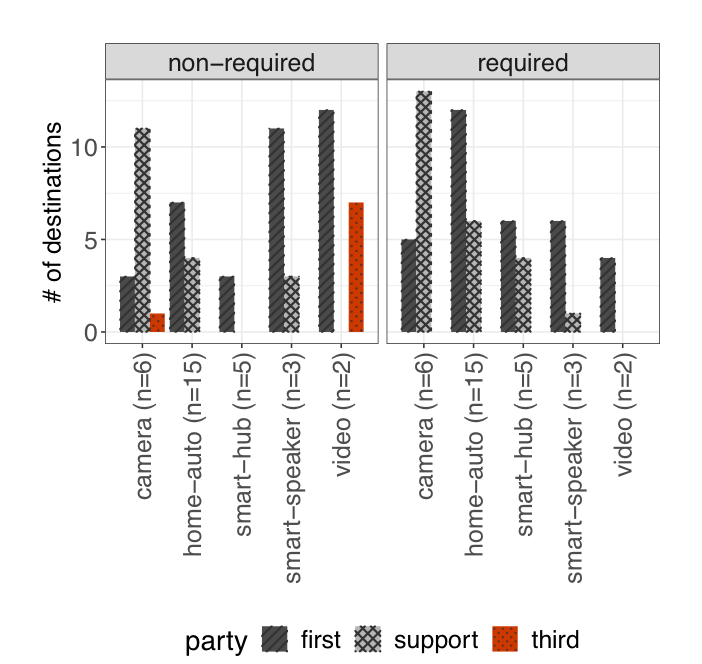
\includegraphics[scale=0.3]{main/pictures/projekt_one/Non_Required_Destination_Per_Party}
    \caption{Ergebnisse der Analyse auf Basis der feingranulareren Einteilung des Netzwerkverkehrs von \textbf{Projekt 1} auf Basis von \cite{Mandalari2021}}
    \label{fig:result-non-req-dest-per-party}
\end{figure}

\noindent Nach der Betrachtung der verwendeten Endpunkte innerhalb von \textbf{Projekt 1} wird der Versuchsaufbau von den 31 Geräten auf eine Grundgesamtheit von 81 Geräten in zwei unterschiedlichen Laboratorien in den USA und UK erweitert. Die zentrale Fragestellung beschäftigt sich hierbei mit der Auswirkung von unterschiedlichen Datenschutzregelungen auf das Verhalten der jeweiligen Geräte und die Art und der Umfang an Daten der durch die Dienstbereitstellung erhoben wird. Des Weiteren wird untersucht, ob sich aus den gesendeten Daten Implikationen auf die Privatsphäre des jeweiligen Nutzers ergeben.

\noindent Grundlegend ist der Versuchsaufbau derselbe geblieben und die Kategorisierung in die drei Endpunkt-Kategorien wurde aus dem vorherigen Projekt übernommen. Eine Erweiterung des Experimentes besteht in der Verknüpfung der beiden Testumgebungen durch einen VPN-Tunnel, um mögliches abweichendes Verhalten der Geräte in Abhängigkeit durch den Standort und somit auch die rechtlichen Regularien zu prüfen. Zudem wurde neben den bereits existierenden fünf Kategorien noch die Kategorie für \textbf{Heimgeräte} wie zum Beispiel Kühlschränke oder Waschmaschinen hinzugefügt, die eine Möglichkeit zur Steuerung über eine Nutzer-Schnittstelle auf dem Smartphone oder dem Web anbieten. Das Auslösen der einzelnen Aktivitäten, wie auch das Messen der Netzwerkaktivität der einzelnen Geräte im nicht benutzten Zustand ähnelt hierbei wieder dem ersten Projekt.

\noindent Auffälligkeiten bezüglich der Ergebnisse aus \textbf{Projekt 2} sind, dass von der allgemeinen Grundgesamtheit 72 Geräte mindestens einen Endpunkt mit Daten versorgen, der nicht zu dem eigentlichen Gerätehersteller gehört. Des Weiteren senden 56\% der Geräte in den USA und 83.3\% in den UK Endpunkte außerhalb ihrer Region. Dieses Verhalten wird nachfolgend durch \ref{fig:traffic_flow} mit der Illustration des ausgehenden Verkehrs von den einzelnen Gerätekategorien in deren Ziel-Länder nochmals übersichtlicher dargestellt.
\begin{figure}
    \centering
    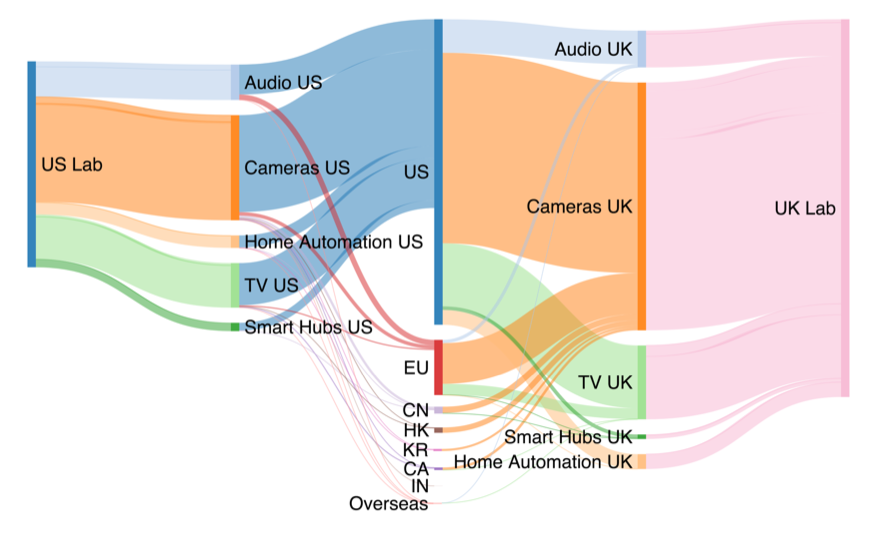
\includegraphics[scale=0.3]{main/pictures/projekt_two/Traffic_Flow_Destinations}
    \caption{Darstellung des Volumens an Netzwerkverkehr ausgehend von den einzelnen Geräten von \textbf{Projekt 2} \cite{Ren2019}}
    \label{fig:taffic_flow}
\end{figure}

\noindent Bezüglich dem Kontaktieren von \textbf{Support-} und \textbf{Third-Parties} wurde ein signifikanter Unterschied zwischen Geräten lokalisiert in den USA und in Europa identifiziert. In den meisten Fällen liegt hierbei die Rate von Geräten innerhalb der USA höher, wie im Vergleich zu ihren europäischen Gegenstücken. Eine genaue Auflistung der Menge an kontaktieren Endpunkten pro Gerätekategorie kann der nachfolgenden Tabelle \ref{table:non-first-party-by-device} entnommen werden. Die Deklarationen $US\cap$ $UK\cap$ beschreiben nur die Geräte, die in beiden Laboren vorkommen und die Deklaration $US \rightarrow UK$ und $UK \rightarrow US$ die Richtung des VPN-Tunnels aus dem jeweiligen Labor.

\begin{table}
    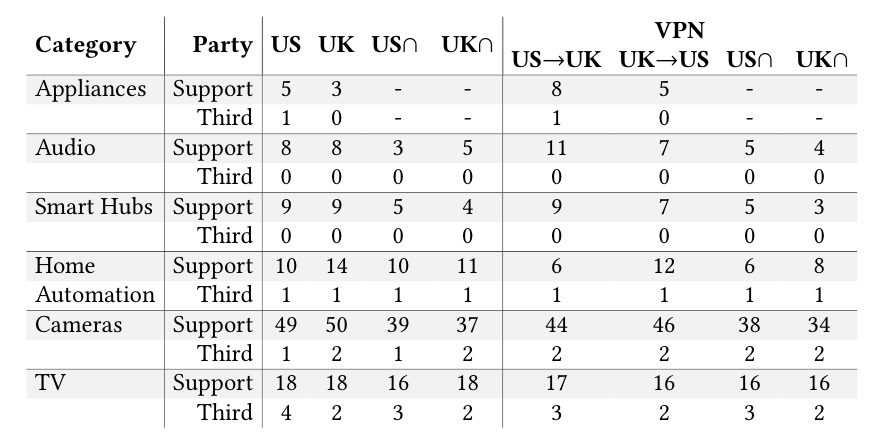
\includegraphics[width=\textwidth]{main/pictures/projekt_two/Non_First_Party_By_Category}
    \caption{Menge an Support- und Third-Parties kontaktiert bei den einzelnen Geräte-Kategorien aus \textbf{Projekt 2} \cite{Ren2019}}
    \label{table:non-first-party-by-device}
\end{table}

\noindent Im Rahmen der Datenanalyse hinsichtlich dem Übertragen von \ac{pii} oder personenbezogenen Daten konnten nur wenige \ac{pii} innerhalb von unverschlüsseltem Netzwerkverkehr festgestellt werden. In vereinzelten Fällen tritt die Preisgabe von Geräte-ID, MAC-Adresse oder diversen UUIDs als unverschlüsselte Nachricht auf. Jedoch besteht bei 30 von 81 Geräten die Möglichkeit durch passives Mitschneiden von erzeugtem Datenfluss eine Rekonstruktion des Nutzerverhaltens, somit eine Kombination aus (User) Tracking und Profiling, durchzuführen. Zusätzlich konnte im Rahmen von unerwartetem Verhalten, das nicht von Nutzer initiiert wurde, bei drei Geräten ein Erhebung von Daten festgestellt werden, die nur teilweise dokumentiert und nicht durch eine Konfiguration des Gerätes durch den Nutzer deaktiviert werden kann. Hierbei handelt es sich nach der Definition der \ac{dsgvo} um personenbezogene Daten, die somit einen hohen Schutzstatus genießen. Die betreffenden Geräte und deren Geräte-Kategorie in Bezug auf deren Eigenheiten werden jedoch nicht als Teil dieser Arbeit genauer betrachtet und können in \cite{Ren2019} recherchiert werden.

%%------------------------------------------------------------------------------------------------
%\subsubsection{Smart City}
%\label{sec:Hauptteil:ssec:Datenerhebung:sssec:Smart City}
%%------------------------------------------------------------------------------------------------

\noindent \textbf{Smart City.}
Wie bereits in der Sektion \fullref{sec:Grundlagen} beschrieben, stellt die \textbf{Smart City} als übergeordneter Kontext den Zusammenschluss aus mehreren \textbf{Smart Environments} dar. Hingegen der Abgeschlossenheit einer \textbf{Smart Home} Umgebung ermöglicht sie, die Aggregation von Daten aus unterschiedlichen Bereichen des urbanen Lebens mit dem Ziel einer Verbesserung der Lebensqualität ihrer Einwohner. Die Konzepte dieses intelligenten Konstruktes beruhen somit auf einer besseren Interkonnektivität ihrer Teilkomponenten und einem daraus resultierenden erhöhtem Datenaustausch \cite{Stefanouli2019}. Diesbezüglich investieren weltweit Städte in den Ausbau und Einsatz von Technologien im Rahmen von Smart City Initiativen, um Problematiken wie zum Beispiel die Nachhaltigkeit hinsichtlich der Umwelt, dem Verkehrsaufkommen innerhalb der Stadt, der Optimierung des öffentlichen Transports und der Gesundheit ihrer Einwohner zu adressieren \cite{BCG2020}.
Jedoch die Datenerhebung jeder einzelnen Applikation oder Systems innerhalb dieses Ökosystems zu analysieren und hinsichtlich ihrer Datenschutzkonformität zu bewerten, ist nicht Teil der hier vorliegenden Arbeit und kann als Bestandteil zukünftiger Forschungsfragen zur Bewertung spezieller Teilbereiche einer \textbf{Smart City} definiert werden. Aus diesem Grunde werden nachfolgend nun zwei Beispiele aus dem Bereich der \textbf{Smart Infrastructure} herausgegriffen, die als Teil der \textbf{Smart City} die auf Echtzeitdaten basierte Regulation des Verkehrs innerhalb einer Stadt zur Aufgabe hat.
 
% Beispiele für Smart City Applikationen

% Erläuterung der BCG Analyse der Traffic App

% Erläuterung der Smart Walk Projekts aus Hamburg

%------------------------------------------------------------------------------------------------
\subsection{Bewertung}
\label{sec:Hauptteil:ssec:Bewertung}
%------------------------------------------------------------------------------------------------


%------------------------------------------------------------------------------------------------
\subsection{Regulationsmöglichkeiten}
\label{sec:Hauptteil:ssec:Regulationsmöglichkeiten}
%------------------------------------------------------------------------------------------------

%%------------------------------------------------------------------------------------------------
%\subsubsection{IoTrimmer \& IoTrigger}
%\label{sec:Hauptteil:ssec:Regulationsmöglichkeiten:sssec:IoTrimmer und IoTrigger}
%%------------------------------------------------------------------------------------------------

% Darstellung des Aufbaus von IoT-Systemen mit anschließender Betrachtung
% der möglichen Regulationen bezüglich der Ansatzstellen

\noindent \textbf{IoTrimmer \& IoTrigger} % Network Layer

%%------------------------------------------------------------------------------------------------
%\subsubsection{IoTInspector}
%\label{sec:Hauptteil:ssec:Regulationsmöglichkeiten:sssec:IoTInspector}
%%------------------------------------------------------------------------------------------------

\noindent \textbf{TODO: IoTInspector oder Smart Walk in Hamburg} % Application Layer

%------------------------------------------------------------------------------------------------
\subsection{Beantwortung der \ac{rq}}
\label{sec:Hauptteil:ssec:Beantwortung der wissenschaftlichen Fragen}
%------------------------------------------------------------------------------------------------

